
\begin{figure}[!h]
  \centering
    \subfloat[压力变化曲线]{
      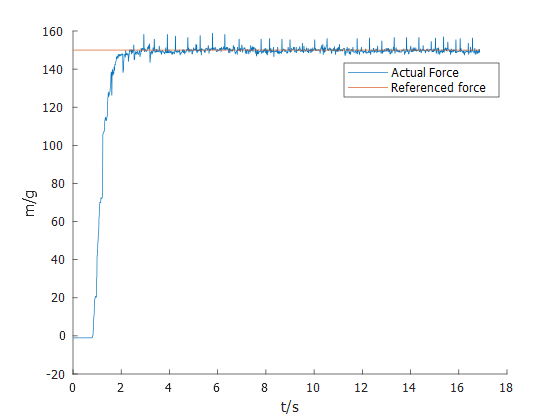
\includegraphics[width=7.2cm]{chapter04/pic/150}
    }
    \hspace{0pt}
    \subfloat[夹爪位置信号]{
      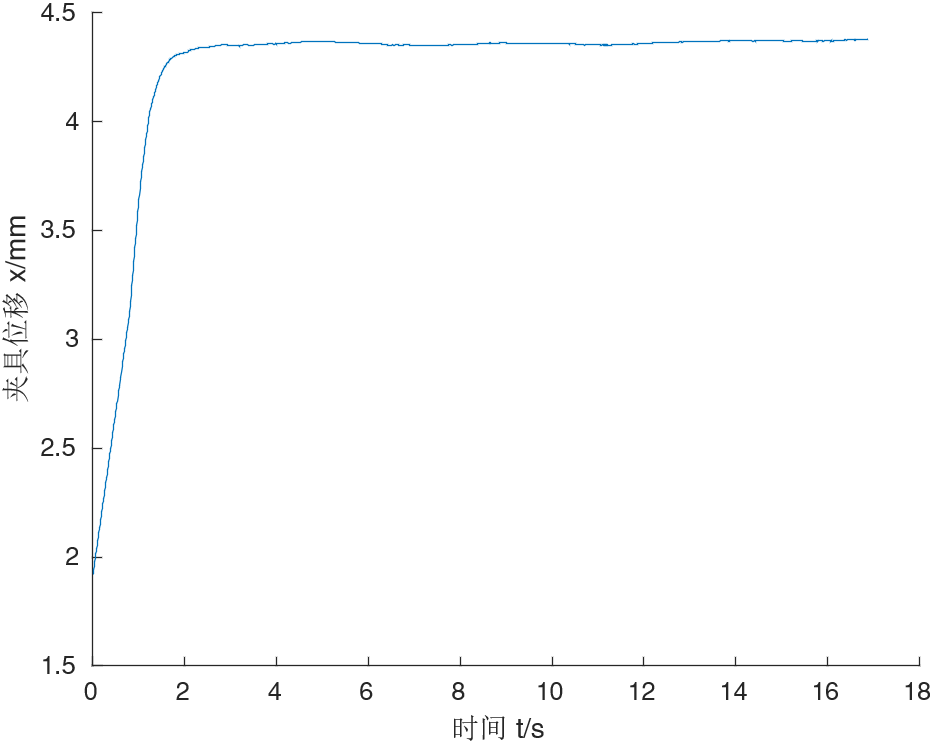
\includegraphics[width=7.2cm]{chapter04/pic/150_x}
    }
  \caption{\label{fig:4-5}阶跃信号下的压力和夹爪位置信号曲线}
  \vspace{-0.3cm}
\end{figure}


\begin{figure}[!h]
  \centering
    \subfloat[压力变化曲线]{
      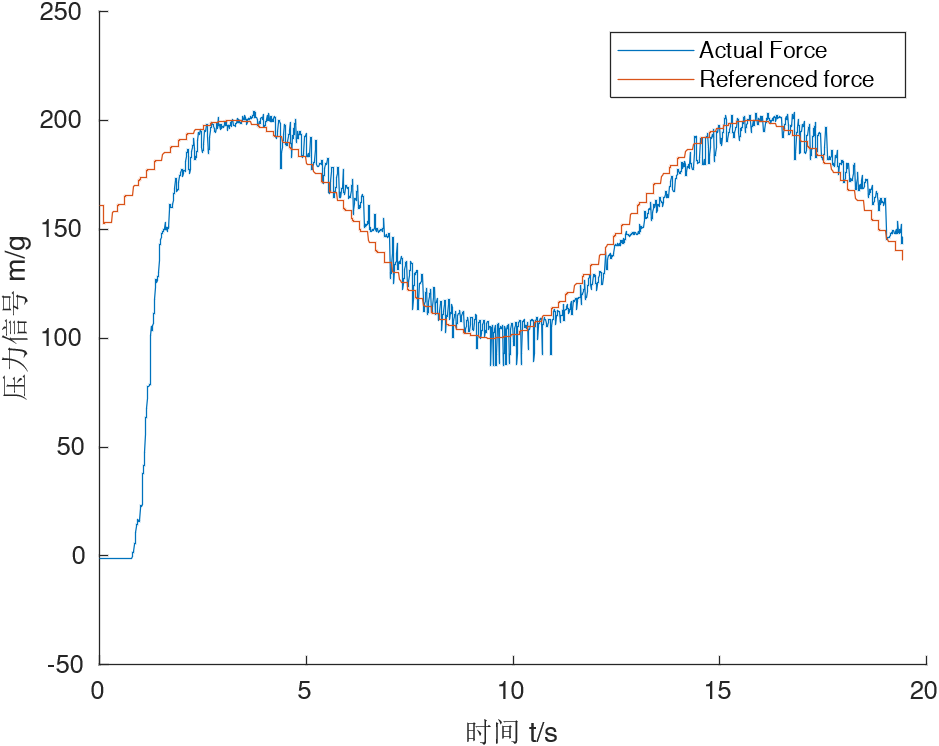
\includegraphics[width=7.2cm]{chapter04/pic/sin}
    }
    \hspace{0pt}
    \subfloat[夹爪位置信号]{
      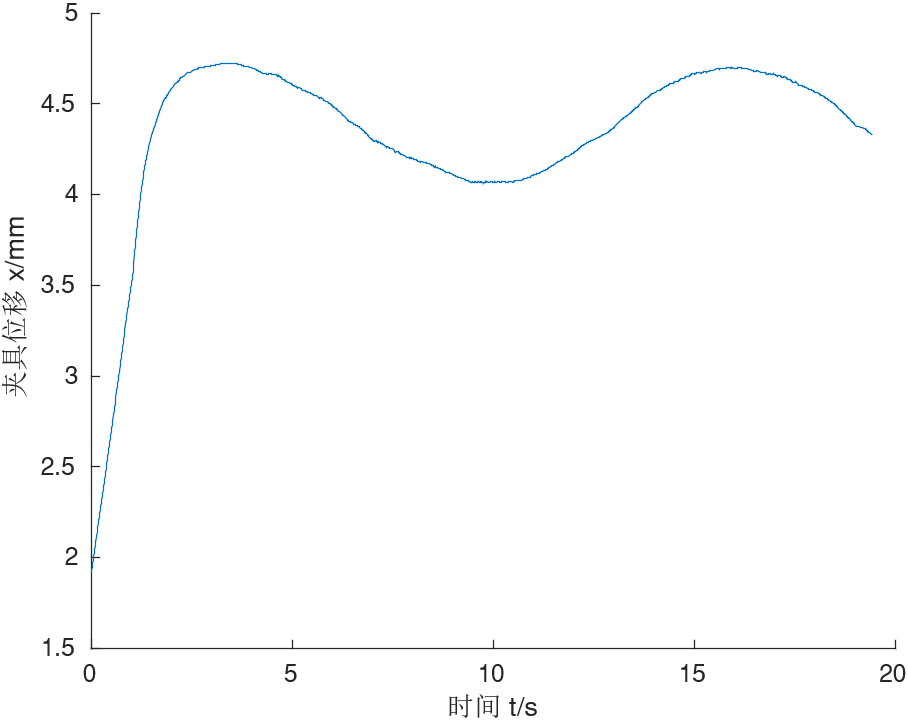
\includegraphics[width=7.2cm]{chapter04/pic/sin_x}
    }
  \caption{\label{fig:4-6}正弦信号下的压力和夹爪位置信号曲线}
  \vspace{-0.3cm}
\end{figure}


\begin{figure}[!h]
  \centering
    \subfloat[夹具位移曲线]{
      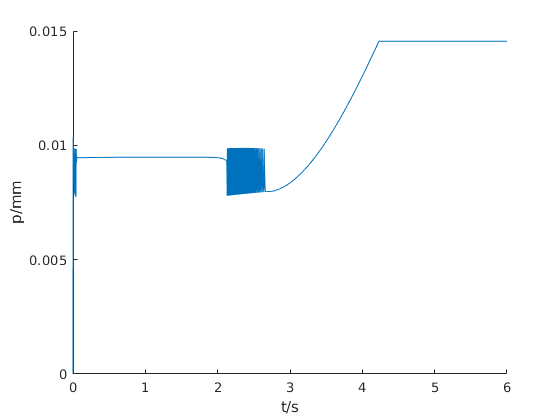
\includegraphics[width=7.2cm]{chapter04/pic/p_f}
    }
    \hspace{0pt}
    \subfloat[压力变化曲线]{
      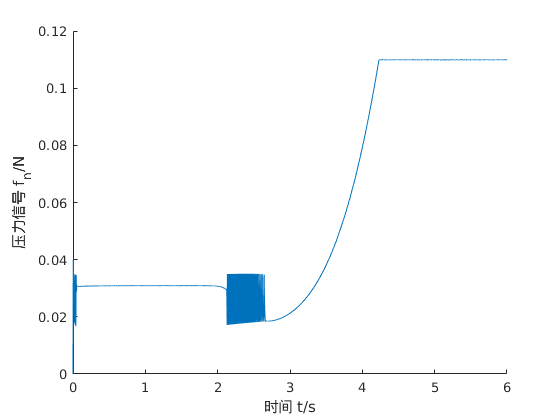
\includegraphics[width=7.2cm]{chapter04/pic/fn_f}
    }
  \caption{夹具位移及受力曲线图}
  \label{fig:4-8}
  \vspace{-0.3cm}
\end{figure}


\begin{figure}[!h]
  \centering
    \subfloat[夹具位移曲线]{
      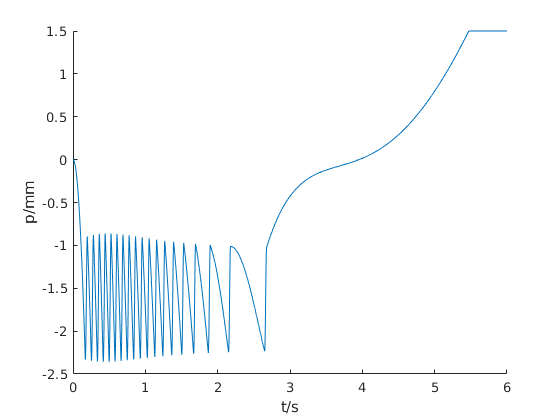
\includegraphics[width=7.2cm]{chapter04/pic/p_x}
    }
    \hspace{0pt}
    \subfloat[压力变化曲线]{
      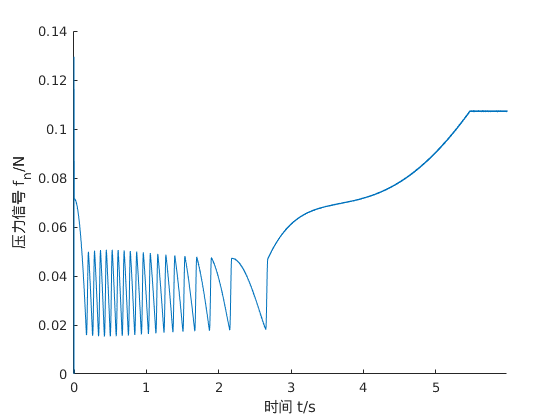
\includegraphics[width=7.2cm]{chapter04/pic/fn_x}
    }
  \caption{夹具位移及受力曲线图}
  \label{fig:4-11}
  \vspace{-0.3cm}
\end{figure}


